\documentclass{article}
\usepackage[utf8]{inputenc}
\usepackage{amsmath}
\usepackage{xcolor}
\usepackage[top=2cm, bottom=2cm, left=2cm, right=2cm]{geometry}
\setlength\parindent{0pt}

\usepackage{listings}
%\usepackage{color}
\usepackage{graphicx}
\usepackage{float}
\usepackage{caption}

\usepackage{verbatim}
\let\oldv\verbatim
\let\oldendv\endverbatim

%\userpackage{minted}

\definecolor{dkgreen}{rgb}{0,0.6,0}
\definecolor{gray}{rgb}{0.5,0.5,0.5}
\definecolor{mauve}{rgb}{0.58,0,0.82}
\definecolor{light-gray}{gray}{0.95}


\lstset{frame=tb,
  language=Java,
  aboveskip=6mm,
  belowskip=6mm,
  showstringspaces=false,
  columns=flexible,
  basicstyle={\small\ttfamily},
  numbers=none,
  numberstyle=\tiny\color{gray},
  keywordstyle=\color{blue},
  commentstyle=\color{dkgreen},
  stringstyle=\color{mauve},
  breaklines=true,
  breakatwhitespace=true,
  tabsize=3,
  backgroundcolor=\color{light-gray},
  language=Matlab
}

%\usepackage{natbib} replaced by line below to make refernces work
\usepackage[square,sort,comma,numbers]{natbib}
\usepackage[nottoc,numbib]{tocbibind} %to get references in table of contants
\usepackage{graphicx}

\usepackage{bm}

\usepackage{hyperref}
\hypersetup{
	colorlinks,
	citecolor=black,
	filecolor=black,
	linkcolor=black,
	urlcolor=black
}

\usepackage{mdframed}
\usepackage{lipsum} % for creating dummy text
\mdfdefinestyle{MyFrame}{%
	linecolor=black,	
	backgroundcolor=gray!20!white,
	skipbelow = 8mm,
	skipabove = 8mm}

\usepackage{scrextend}

\title{Fys4150\\Project 1\\ }
\author{Peter Killingstad and Karl Jacobsen}


\begin{document}
	
\maketitle

\tableofcontents

\pagebreak
\section{Abstract}

\section{Introduction}
Goals: Learn C++, dynamic memory allocation, discretizing differential equations and setting up a linear system, algorithms for solving tridiagonal linear systems, error-analysis (truncation and precision), efficiency analysis.

\section{Theory}


\subsection{Setting up the linear system}
In this project we will solve the one-dimensional Poisson equation
with Dirichlet boundary conditions by rewriting it as a set of linear equations.


To be more explicit we will solve the equation

\begin{equation}\
-u''(x) = f(x), \hspace{0.5cm} x\in(0,1), \hspace{0.5cm} u(0) = u(1) = 0.
\end{equation}

\begin{equation}
-u''(x) = f(x), \hspace{0.5cm} x\in(0,1), \hspace{0.5cm} u(0) = u(1) = 0.
\label{eqn:diffEquation}
\end{equation}

and we define the discretized approximation  to $u$ as $v_i$  with 
grid points $x_i=ih$   in the interval from $x_0=0$ to $x_{n+1}=1$.
The step length or spacing is defined as $h=1/(n+1)$. 
We have then the boundary conditions $v_0 = v_{n+1} = 0$.
We  approximate the second
derivative of $u$ with

\begin{equation}
-\frac{v_{i+1}+v_{i-1}-2v_i}{h^2} = f_i  \hspace{0.5cm} \mathrm{for} \hspace{0.1cm} i=1,\dots, n,
\label{eqn:discretizeEquation}
\end{equation}
where $f_i=f(x_i)$. \\

Now we will show that the discrete problem can be rewritten to a linear system of the type 

\begin{equation*}
\mathbf{A}\mathbf{v} = \tilde{\mathbf{b}}.
\end{equation*}

The reason for wanting the rewrite to a linear system, is that we know of methods that solve such linear systems. Hence, by solving the linear system we will also solve our discrete differential equation problem!\\

To obtain the linear system, we can write out the discretized approximation into a system of equations. We start by setting $i=1$, multiply the discretize equation (\ref{eqn:discretizeEquation}) with $h^2$ and write out the first couple of equations to look for a pattern

\begin{eqnarray}
\nonumber
-2v_1 + v_2 &=& f_1h^2 \\ \nonumber
v_1 - 2v_2 +v_3 &=& f_2h^2 \\ \nonumber
v_2 - 2v_1 +v_4 &=& f_3h^2 \\ \nonumber
v_3 - 2v_2 +v_5 &=& f_4h^2 \\ \nonumber
\vdots &=& \vdots \\ \nonumber
v_{n-1} - 2v_n &=& f_nh^2. \\ \nonumber
\end{eqnarray}

As the equation is written out, it is clear that the values $1, -2$ and $1$ is repeating. We can now rewrite the system of equations into a matrix made up of the coefficients and two vectors, one containing the unknowns $v_1$ to $v_{n}$ and the other containing the inhomogeneous terms $f_1$ to $f_{n}$. The system would then be 

\begin{equation}
\underbrace{\begin{bmatrix} -2 & 1 & \cdots & 0 \\ 1 & -2 & 1 & \vdots \\
\vdots & &  \ddots & \vdots \\ 
0 & \cdots & 1 & -2 \end{bmatrix}}_{\mathbf{A}} 
\underbrace{\begin{bmatrix} v_1\\ v_2 \\ \vdots\\ v_n \end{bmatrix}}_{\mathbf{V}} = 
\underbrace{\begin{bmatrix} f_1 h^2\\ f_2 h^2 \\ \vdots \\ f_nh^2\end{bmatrix}}_{\mathbf{\tilde{b}}}
\end{equation}

\subsection{Linear system solvers}


\subsubsection{Gaussian elimination tridiagonal systems}
We use standard Gaussian elimination, utlizing the sparsity of the matrix by ignoring the zero terms when doing the forward and backward substitution. This gives the Thomas algorithm. The algorithm can be seen in our code, which follows:

\begin{lstlisting}
void gaussianTridiagonalSolver(double ** computed_tridiagonal_matrix, double * computed_right_hand_side, double * computed_numerical_solution, int N){
double multiplicationFactor;
for (int i = 1; i < N; i++){
multiplicationFactor = computed_tridiagonal_matrix[i][i-1]/computed_tridiagonal_matrix[i-1][i-1];
computed_tridiagonal_matrix[i][i-1] = 0;
computed_tridiagonal_matrix[i][i] += - multiplicationFactor*computed_tridiagonal_matrix[i-1][i];
computed_right_hand_side[i] += - multiplicationFactor*computed_right_hand_side[i-1];
}
for(int i = N-1; i > -1; i--){
if(i == N-1)
computed_numerical_solution[i] = computed_right_hand_side[i];
else
computed_numerical_solution[i] = computed_right_hand_side[i+1] - computed_tridiagonal_matrix[i][i+1]*computed_numerical_solution[i+1]/computed_tridiagonal_matrix[i][i];
}

}
\end{lstlisting}

\textbf{Task 2} We can insert a few comments in the top of the function, explaining the algorithm. \\

Now we want to calculate the number of floating points operations (FLOPS) needed to solve the linear system with the above algorithm. This is an extremely important topic, since the number of FLOPS typically will be very large in physics problems, and having an algorithm that reduces the FLOPS can be the difference between being able to solve the problem and not!\\

According to Wikipedia, the Thomas algorithm requires $\mathcal{O}(n)$ FLOPS. To check our understanding, we will try calculating the number of FLOPS ourself. Looking at the code above, we start by caunting FLOPS in the forward substitution, which is the first for loop. The variable 'mutliplicationfactor' equals a division, which counts as one FLOP. '\texttt{coputed\_tridiagonal\_matrix}' enveolves a sum of two terms, which gives one FLOP, and a multiplication, which gives another FLOP. So in total for '\texttt{computed\_tridiagonal\_matrix}' we have 2 FLOPS. Next the calculation of '\texttt{computed\_right\_hand\_side}' envolves a multiplication (1 FLOP) and a summation (1 FLOP), giving 2 FLOPS for '\texttt{computed\_right\_hand\_side}'. For each iteration in the loop, we have a total of 5 FLOPS. The loop goes from $1$ to $N-1$, giving $N-1$ iterations. This, in total we have $5(N-1)$ FLOPS, which is equal to $\mathcal{O}(N)$ FLOPS, which is the same as given on Wikipedia.

\subsubsection{Gaussian elimination symmetric tridiagonal systems}
If the tridiagonal system is symmetric, $A = A^T$, the Gaussian elimination method can be made even simpler than in the Thomas algorithm. The program below shows the algorithm and its implementation.

\begin{lstlisting}
void gassianTridiagonalSymmetricSolver(double ** computed_tridiagonal_matrix, double * computed_right_hand_side, double * computed_numerical_solution, int N){
for (int i = 1 ; i < N; i++){
computed_tridiagonal_matrix[i][i] += -computed_tridiagonal_matrix[i-1][i]*computed_tridiagonal_matrix[i-1][i]/computed_tridiagonal_matrix[i-1][i-1];
computed_right_hand_side[i] += -computed_tridiagonal_matrix[i-1][i]*computed_right_hand_side[i-1]/computed_tridiagonal_matrix[i-1][i-1];
}

computed_numerical_solution[N-1] = computed_right_hand_side[N-1]/computed_tridiagonal_matrix[N-1][N-1];
for (int i = N-2; i > -1; i--){
computed_numerical_solution[i] = computed_right_hand_side[i] - computed_tridiagonal_matrix[i][i+1]*computed_numerical_solution[i+1]/computed_tridiagonal_matrix[i+1][i+1];
}
}
\end{lstlisting}

\textbf{Task 4} The above listing must be made more pretty bby fixing the spaces, but that can wait tuil we know we have the final program. Also for this function, we should in the top add lines describing the algorithm.\\

\textbf{Task 5} Here we should do, and show, FLOP-count for the above listed algorithm.

\subsubsection{LU}
We will compare the speed of our algorithms with the speed of the LU-algorithm. According to Hjorth-Jensen \cite{MHJ} p. 173, solving a system with LU is $\mathcal{O}(n^2)$ requires FLOPS, but the composition itself requires  $\mathcal{O}(n^3)$ FLOPS. Based on this, we expect our algorithms to outperform the LU-algorithm, independentlyu of whether one includes the composition itself in the comparison or not.\\

Here we will try ourself to compute the FLOP requirements for solving a system with LU. One starts by solving $Ly = w$ for $y$, where L is lower tridiagonal $N\; X\; N$ with 1 on the diagonal. Seting up the first few iterations of the loop solving the system, we hopefully see a pattern:
\begin{align}
y_1 &= w_1\\
y_2 &= w_2 - L_{21} y_1\\
y_3 &= w_3 - L_{31} y_1 - L_{32}y_2\\
\vdots\\
y_{N}& = w_N - \sum_{i}^{N-1} L_{Ni} y_i
\end{align}

\subsection{Error calculations}
Having knowledge about the errors of the numerical solutions is essential, because without this knowledge, it is difficult to know the validity of the results. Without knowledge of validity of the results, we are exiting the subject of (natural) science. \\

Leaving out probably the largest error source, our selves, there will be two possible sources of errors: truncation error due to numerical approximation of continuous operators (the 2nd derivative), and round-off errors due to limited computer precision. Below we will derive some expressions for these errors, giving us knowledge about what to expect from the numerical solutions.

\subsubsection{Truncation error}

In our differential equation, we approximate the 2nd derivative with a truncated Taylor-polynomial. A nice thing by using Taylor ploynomials is that we have knowledge about the truncation error, the difference between numerical and exact solution due to terms in the Taylor series being left out. It turns out that in our case the truncation error depends on the step size, $h$. Hence we know what to expect of the truncation error when varying $h$. \\

In our case the truncation error is of $\mathcal{O}(h^2)$. From this we expect the truncation error to depend on the step lenght, $h$, to a order of 2, meaning that a reduction of $h$ by a factor of 10 should reduce the truncation error by a factor of 20.

\subsubsection{Round-off errors}
\textbf{Task 6} Write something about this.

\subsubsection{Total error}
We are more interested in the relative error, meaning the difference between the numerical and exact solution, relateive to the exact solution, than in the pure error. The reason for this, is that a small pure error could be physically insignificant if the quantities are big, while on the other hand a small pure error could be very significant if the quantities we are measuring are small. Example: 1 cm in error when simulating trajectories of planets is probably less physically significant than 1 cm error when doing simulations on molecular level.\\

For inspection of errors, and relating them to the expected convergence rates from Taylor series theory, it is neat to take the log the the errors and of the step lengths. Plotting this, the slopes could be directly compared with the expected convergence rate, the $\mathcal{O}$-term from the Taylor approximation of the 2nd derivative.\\

Our solutions will be vectors, so there will be errors at each vector element. We are interested in a rough error-number, so we want an error measure that represents all of the array-points. One way of doing this, is for each step length to extract the max value of the relative error. By this method, we know that the error we get is an upper bound for all local errors, local meaning errors at the different vector elements.\\

By the methods mentioned above, we compute the relative error in the data set $i=1,\dots, n$,by setting up

\[
\epsilon_i=log_{10}\left(\left|\frac{v_i-u_i}
{u_i}\right|\right),
\]
as function of $log_{10}(h)$ for the function values $u_i$ and $v_i$, and extract the maximum for each step length.

\section{Results}

\subsection{Efficiency}
The below table displays the times used by the different algorithms. Not that the LU-time includes also the time for the LU-decomposition, in addition to the time solving the system.

\lstset{backgroundcolor=\color{white}}
\begin{minipage}{.32\textwidth} %\noindent
	\lstinputlisting[language={},title={Tridiagonal
	}]{/home/karl/doc/subj/att/fys4150/project1/cpuTimeTridiagonal.tex}
\end{minipage}\hfill
\begin{minipage}{.32\textwidth}
	\lstinputlisting[language={},title={Symmetric
	}]{/home/karl/doc/subj/att/fys4150/project1/cpuTimeTridiagonalSymmetric.tex}
\end{minipage}\hfill
\begin{minipage}{.32\textwidth}
	\lstinputlisting[language={},title={LU
	}]{/home/karl/doc/subj/att/fys4150/project1/cpuTimeLU.tex}
\end{minipage}\hfill

From the above table we that LU clearly uses more time than the other algorithms. This is in according to expectations, knowing that LU should be $\mathcal{O}(N^3)$ in FLOPS, while at least the tridiagaonal solver should be $\mathcal{O}(N)$ FLOPS.\\

The figure below may perhaps give a better impression on the times for the different algorithms, at least on how the results compare to the theoretical FLOP-estimations.

\begin{figure}[H]
	\centering
	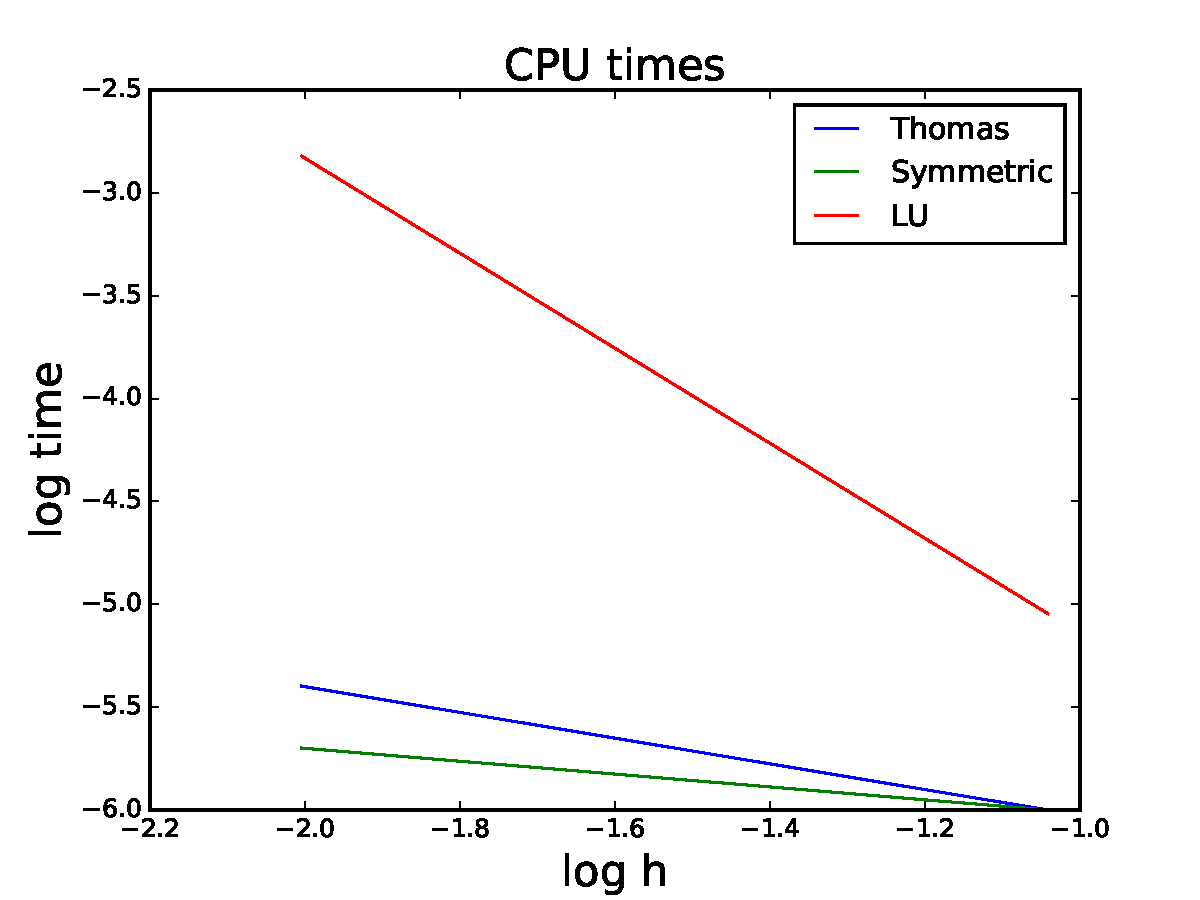
\includegraphics[width=0.99\textwidth]{/home/karl/doc/subj/att/fys4150/build-project1qt-Desktop_Qt_5_9_1_GCC_64bit-Debug/logTimes.pdf}
	\caption{Log CPU-times}
	%\label{1}
\end{figure}

The figure above shows that the Thomas algorithm is $\mathcal{O}(N)$, the incline is about $-1$ in the figure. For the LU we get a slope somewhere between 2 and 3. Knowing that the decomposition is of order 3 and the solution of the system by LU is of order 2, we had expected an incline of 3 in our graph, since the largest $N$ should dominate. We are not sure why we do not get a slope of 3 for LU. \\

We were asked if it would be possible to run LU for $N=10^5.$ From before, we know that the Thomas algorithm, which is $\mathcal{O}(N)$, makes the computed crash for $N = 10^6$. Solving LU, which is $\mathcal{O}(N^3)$ for $N = 10^5$, would give FLOPS of order $10^15$, which would never be solved on our computer.

\subsection{Error analysis}
The below table shows the errors for LU and the Thomas algorithm. It was expected that these two algorithms should produce results equal to each other, whithin machine precision. Both algorithms solves exactly the same system. The table below confirms our expectation. However, we suspect that there could have appeared larger errors, due to numerical issues, knowing e.g. that zeros in matrices can cause trouble.

\lstset{backgroundcolor=\color{white}}
\begin{minipage}{.49\textwidth} %\noindent
	\lstinputlisting[language={},title={LU
	}]{/home/karl/doc/subj/att/fys4150/project1/errorLu.txt}
\end{minipage}\hfill
\begin{minipage}{.49\textwidth}
	\lstinputlisting[language={},title={Thomas
	}]{/home/karl/doc/subj/att/fys4150/project1/errorTridiagonal.txt}
\end{minipage}\hfill

Since the algorithms give the same error, we use only the results from one of the algorithms when analysing the error. The below figure shows the numerical results from the Thomas algorithm and the exact solution.

\begin{figure}[H]
	\centering
	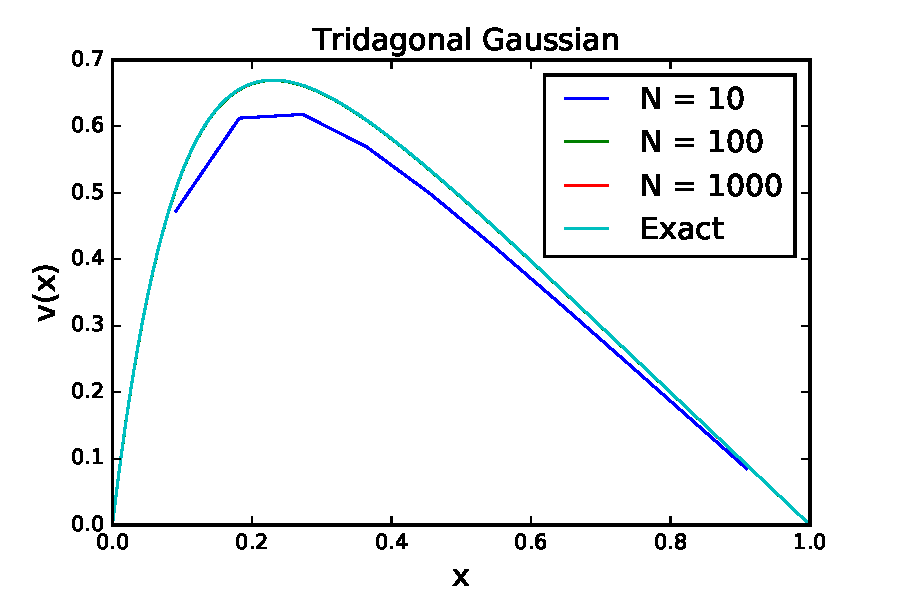
\includegraphics[width=0.99\textwidth]{/home/karl/doc/subj/att/fys4150/build-project1qt-Desktop_Qt_5_9_1_GCC_64bit-Debug/gaussianTridiagonal_comparison.pdf}
	\caption{Results Tridiagonal Gaussian}
	%\label{1}
\end{figure}

We see that except for the coarsest grid, $N=10$, the fit is really good. Knowing that our approximator for the 2nd derivative is 2nd order, and the fact that the simulations in the figure has 10, 100 and 1000 grid points, it is not surprising that the error is reduced considerably when the grid is made 10 times finser in each step. With a convergence rate of 2, a ten fold refinement in the grid should lead to a 100 fold refinement in the truncation error.\\

Below follows figures for the relative error. Not that the scales on the x-axis on the two figures are not the same. The reason for different scale is that our computed crashed when we increased N tenfold from the last N in the right figure.\\


\begin{minipage}{.49\textwidth} %\noindent
\begin{figure}[H]
	\centering
	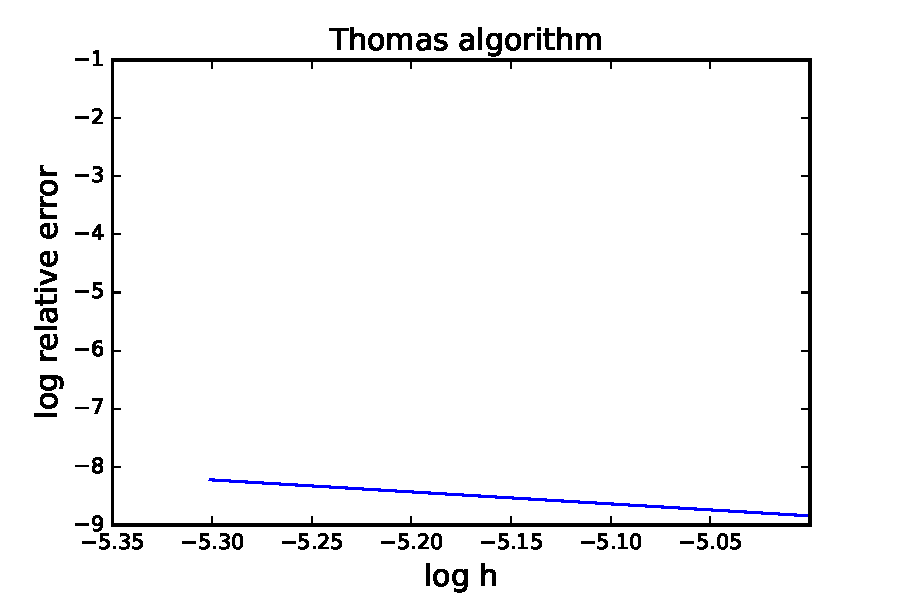
\includegraphics[width=0.99\textwidth]{/home/karl/doc/subj/att/fys4150/build-project1qt-Desktop_Qt_5_9_1_GCC_64bit-Debug/gaussianTridiagonal_error2.pdf}
	\caption{Results Tridiagonal Gaussian}
	\label{1}
\end{figure}
\end{minipage}\hfill
\begin{minipage}{.49\textwidth}
\begin{figure}[H]
	\centering
	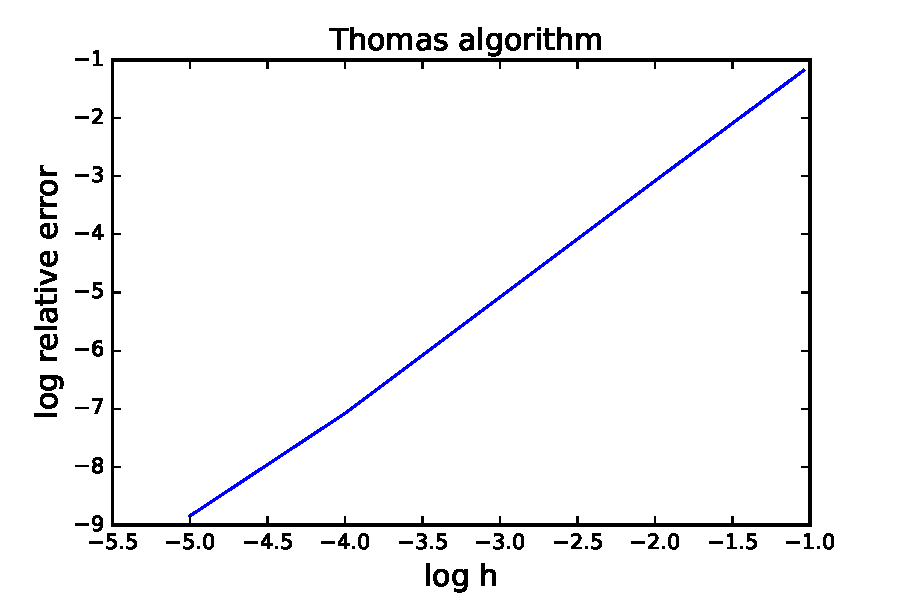
\includegraphics[width=0.99\textwidth]{/home/karl/doc/subj/att/fys4150/build-project1qt-Desktop_Qt_5_9_1_GCC_64bit-Debug/gaussianTridiagonal_error.pdf}
	\caption{Results Tridiagonal Gaussian}
	\label{1}
\end{figure}

\end{minipage}\hfill

Our computer crashes for $N = 10^6$, so the above figure to the right stops at $N = 10^5$. The figure shows that up to $N = 10^5$, the error seems to follow the expected truncation error, since the slope seems to be pretty close to 2.\\

The figure to the left above shows the error-development staring where the previous figure left off, but with smaller increases in $N$.\\

\textbf{task 10} Comment uppon the error (truncation verson round-off). Where to expect turning point....






\section{Conclusions}
\textbf{Task 13} Sum up the results here.

\section{Feedback}
\textbf{Task 14} What has been good, something that could have been done better?

\begin{thebibliography}{9}
	\bibitem{MHJ} 
	Hjorth-Jensen, M.(2015)
	\textit{Computational physics. Lectures fall 2015}. 
	\url{https://github.com/CompPhysics/ComputationalPhysics/tree/master/doc/Lectures}
\end{thebibliography}


\end{document}
